\section{System Model}

\subsection{Conventional Task Model}
%\subsection{Task Model}
The directed acyclic graph (DAG) model of hard real-time
tasks~\cite{li2014analysis} defines the set of ${n}$ sporadic tasks ${\tau}$ as
${\tau = \{\tau_1,\tau_2, ..., \tau_n\}}$. A task ${\tau_i}$
in the task system generates a potentially infinite number of jobs,
each arriving no less than ${T_i}$ time units after the previous
job with deadline ${D_i}$ constrained by the task's period
${D_i \leq T_i}$. Each parallel task ${\tau_i \in \tau}$
is represented by a DAG ${G_i}$. The set of ${n}$ DAGs is
denoted ${\mathbb{G} = \{G_1, G_2, ..., G_n\}}$.

\begin{figure}[!h]
  \centering
  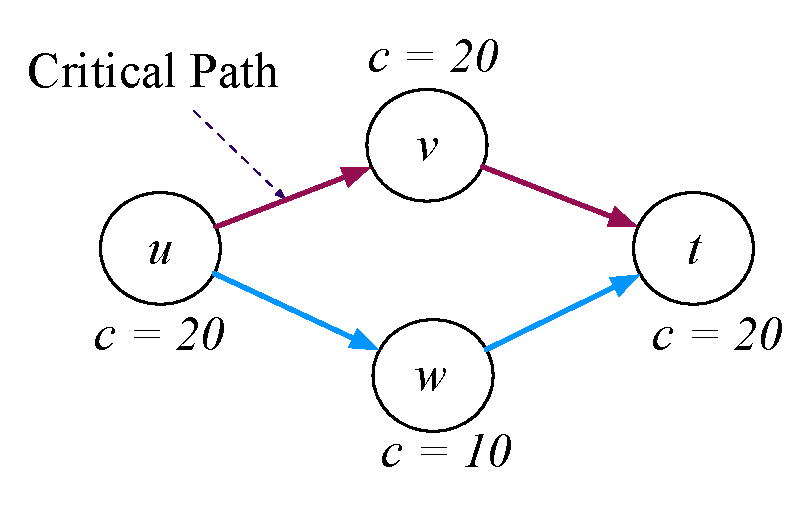
\includegraphics[width=0.4\columnwidth]{dag}
  \caption{An Example of a Parallel Real-time Task}
  \label{fig:dag}
\end{figure}
  
  \revise{Mathmode for labels: the WCET uses a different typeset
${\mathrm{c_v}}$ and font. It should follow the typesetting and
font of the rest of the paper ${c_v}$}


Each node ${v \in V_i}$ of a DAG ${G_i =
  (V_i, E_i)}$ represents the 
execution of a thread and an edge ${e \in E_i}$ represents a
dependency between two nodes. A dependency between two nodes indicates
that a node is ready to execute only upon the completion of all its
predecessor nodes. The conventional model considers a source as a node with no incoming
arcs and a sink as node with no outgoing arcs. For the sake of
simplicity, the conventional model assumes a task has only one source and sink node. In
practice, this not hard to achieve as a source and sink can be added
to the task with $0$ execution and not change the task dependencies.

Nodes of a task have an associated worst-case execution time. 
An example of the DAG task is shown in Fig.~\ref{fig:dag}. Node $v$ represents a single thread execution which requires a worst-case execution time of $20$ time units. A directed edge between node $u$and $v$ denotes node $v$ can be released for execution only after the completion of node $u$.

%%\revise{For a node $v \in V_1$, we define the function $\parent{\node{1}}$ as the set of parent nodes of node $\node{1}$, i.e., node $\node{1}$ is executed only after the successful completion of all the nodes in $\parent{\node{1}}$.  The function $\child{\node{1}}$ is defined as the set of child nodes of $\node{1}j$, i.e., all nodes in the set given by $\child{\node{1}}$ cannot be released before node $\node{1}$ completes execution. We define $\pred{\node{1}}$ and $\successor{\node{1}}$ as a set of all predecessors of $\node{1}$ and a set of all successors of $\node{1}$, respectively.}

A node $v \in V_i$ is said to be dependent on $u \in V_i$ , if there is a path from $u$ to $v$ of some arbitrary length in the DAG $G_i$. This dependency is expressed as \textbf{${u \prec^* v}$}, where $\prec^*$ indicates the dependency and $*$ denotes an arbitrary length. Similarly, a path between two nodes $u, v \in V$ of a DAG $G_i$ is represented by $u \prec^{x} v$, where $x$ denotes the length of the path. For example, $u \prec^{3} v$ denotes that there exists a path from $u$ to $v$ of length of 3.
For any given task, the work in~\cite{li2014analysis} defines \textit{critical path} $\lambda_i$ of a 
task $\tau_i$ as the longest execution time path that starts from
source and ends at the sink. \textit{Critical path length} ($\L_i$) is
defined as the sum of execution times of all nodes along the critical
path $\lambda_i$ of task $\tau_{i}$.  Workload $C_{i}$ of
a task $\tau_{i}$ is defined as the sum of worst-case execution time of
all nodes in the DAG task. 

\subsection{Federated Scheduler}
For a task set $\tau$ , the federated scheduling algorithm proposed in~\cite{li2014analysis} works as
follows. The task sets is divided into two disjoint sets
$\tau_{high}$  and $\tau_{low}$. $\tau_{high}$ contains all tasks with
high utilization (i.e. $u_i > 1$) and $\tau_{low}$ contains all
remaining low utilization tasks. Each task in $\tau_{high}$ is
assigned $m_{i}$ dedicated cores (no other task is executed on these
cores), where: \begin{equation}\label{eq:m} m_{i} = \left\lceil \frac{C_{i} - L_{i}}{D_{i} - L_{i}}
\right\rceil \end{equation}

\noindent The total
number of cores assigned to high-utilization tasks is denoted as $m_{high} = \sum_{\tau_{i} \in \tau{high}} m_{i}$. 
The remaining cores to all low-utilization tasks in $\tau{low}$, denoted
as ${m_{low} =  \mathbb{m} - m_{high}}$. The federated scheduling algorithm admits
the task set ${\tau}$, if $m_{low}$ is non-negative and all tasks in
$\tau_{low}$ are schedulable sequentially.  

After a valid core allocation, runtime scheduling proceeds as
follows. Any greedy (work-conserving) parallel scheduler can be used
to schedule a high-utilization task $\tau_{i} \in \tau_{high}$ on its
assigned $m_{i}$ cores. Informally, a greedy scheduler is one that never
keeps a core idle if some node is ready to execute. 

All low-utilization tasks are treated and executed as though they are
sequential tasks and any multiprocessor scheduling algorithm (such as
partitioned EDF, or various rate-monotonic schedulers) can be used to
schedule all the low-utilization tasks on the allocated $m_{low}$
cores. The federated scheduler treats all low-utilization tasks as sequential tasks
since $C_{i} \le D_{i}$ and parallel execution is not required to meet their
deadlines. 

\subsection{Processing Model}

In this work, for each core, we assume a dedicated direct mapped
instruction cache. We assume a time-compositional architecture\addcite,
where memory and execution demand are separable. Copying a block of 
main memory to cache memory requires $\brt$ cycles, commonly
referred to as the the block reload time (BRT). If multiple cores share
the same processing platform their cache contents do not interfere with
one another. The impact of a shared cache between cores is not considered.


\subsection{Proposed Changes to the Conventional Task Model}
Here, we discuss the proposed changes to the task model and processing model used in this paper.
For the rest of the paper, we work with one DAG task at a time, and hence we drop the subscript notation.
For a DAG ${G = (V, E)}$ representing a parallel task, each node ${v \in V}$ represents
the release, execution, and termination of a single thread within one task 
\cite{li2014analysis}. In the existing model, the only relationship between thread releases and the executable object they execute is the worst-case execution time of the node. Two nodes ${u, v \in V}$ may represent two threads executing the same object (possibly on different processors).

To take advantage of instruction cache reuse, we propose a simple modification to the DAG
model. Where possible, distinct nodes that represent the execution of
the same object are collapsed into a single node. To accommodate collapse,
nodes are identified by their executable object, and a new attribute is added to every node
indicating the number of threads which will be executed over the object.

In the conventional model~\cite{li2014analysis}, each node ${v \in V}$ is characterized
with a single worst case execution time for a single thread. We
propose that each node's WCET is characterized by a function
${c_{v}(\eta_{v})}$ where $\eta_{v}$ is the number of threads that will execute the
node ${v}$ on the same core serially (one after another) with no
other thread executing a different object on the core in between executions.

In this work, a node ${v \in V}$ is represented by a tuple ${v = \langle \alpha_{v}, c_{v}(\eta_{v}), \eta_{v} \rangle }$, where $\alpha_{v}$ is the code segment the thread executes, $\eta_{v}$ is the number of threads, and ${c_{v}}$ is the WCET function for ${\eta_v}$ threads. The proposed model is  compatible with the previous model \cite{li2014analysis} where the previous model can be expressed as ${v = <\alpha_{v}, c_{v}(\eta_v), \eta_v=1>}$. Note that, we will discuss the computation of $c_{v}(\eta_{v})$ in a later section.

\begin{figure}
  \centering
  \begin{subfigure}[b]{0.4\textwidth}{
      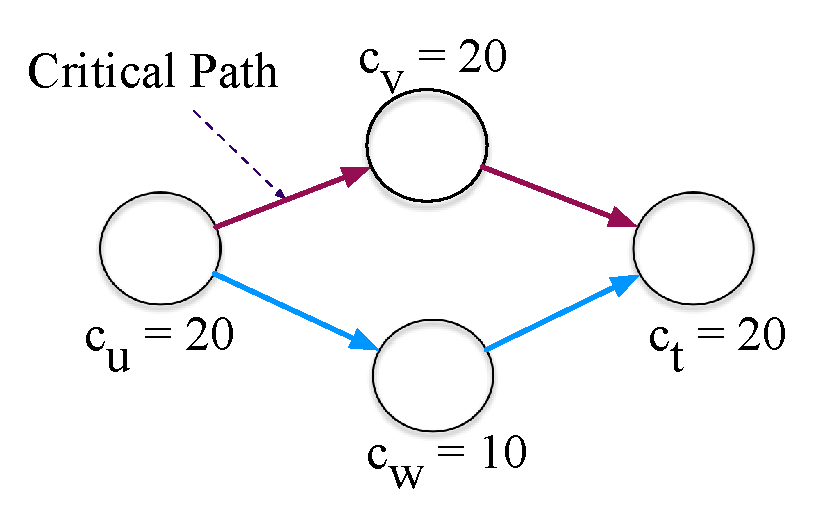
\includegraphics[width=\textwidth]{existingDAGmodel}
      \caption{Existing DAG model}
      \label{fig:existingDAGmodel}
    }
  \end{subfigure} \quad
  \begin{subfigure}[b]{0.4\textwidth}{
      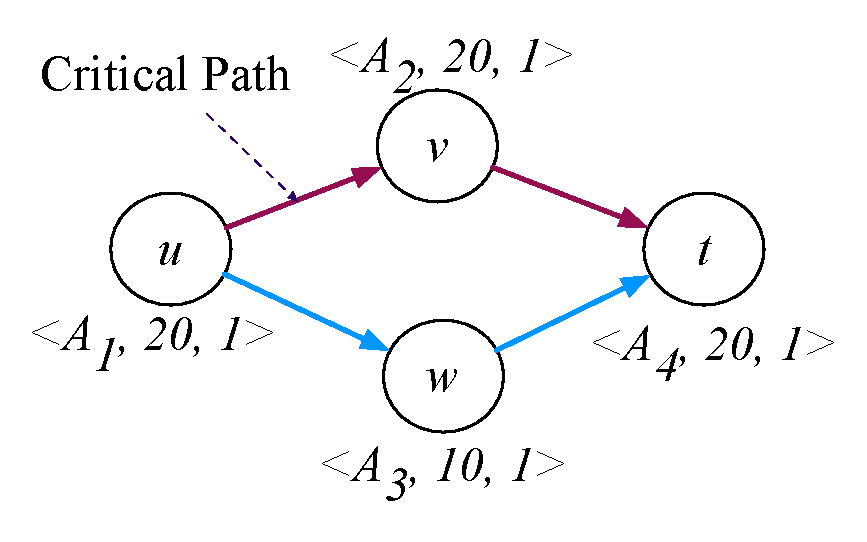
\includegraphics[width=\textwidth]{proposedDAGmodel}
      \caption{Proposed DAG model}
      \label{fig:proposedDAGmodel}
    }
  \end{subfigure}
  \caption{Proposed changes to the DAG model}
  \label{fig:dag-change}
\end{figure}


Fig.~\ref{fig:dag-change} highlights the proposed changes to the DAG task model.  Node $v$ in Fig.~\ref{fig:existingDAGmodel} represents a single thread execution which requires a worst-case execution time of $20$ time units. In the proposed model, we represent node $v$ as a tuple $v : \langle \alpha_v = B, c_v(\eta_v) = 20,  \eta_v = 1\rangle$, where $B$ refers to a unique code segment, $ c_v(\eta_v)$ refers to the worst-case execution time of $1$ thread which is $20$ time units, and $\eta_v$ refers to the number of threads which is 1.

 A goal of this work is to bring the inter-thread cache benefit \addcite to parallel DAG tasks. 

%% ct - commented out because splitting a code segment into multiple code segments may introduce loops in the DAG. 
%%		For example, if a loop is too big and cannot fit into a cache block then we it will be split across multiple segments which will introduce a DAG.
%%
%%A goal of this work is to bring the inter-thread cache benefit \addcite to parallel DAG tasks. As a first-step, two requirements are placed on nodes of the graph.
%%\begin{description}
%%\item[R1] All executable objects must fit entirely within the cache.
%%\item[R2] No two instructions of an executable object may evict one another.
%%\end{description}
%%
%%Requirements R1 and R2 may be met for any executable object by repeatedly dividing
%%the object source that result in objects larger than the cache into separate code segments, carefully recompiling those code segments to maximize cache use, and replacing the original node with a serial set of nodes.
%%\\
%%\\
%%\emph{ct-3 A figure is needed to illustrate the transformation from one over-sized node, to multiple correctly sized nodes}
%%\\



%%Given a timing-compositional architecture with the restrictions \textbf{R1} and \textbf{R2},
%%${c_i(n)}$ can be expressed for any node in terms of the memory demand of all instructions
%%of ${v_j \in V_i}$ into the cache ${\gamma_j}$ and the worst-case execution demand
%%to execute the node assuming all instructions of ${v_j}$ have
%%been cached ${\iota_j}$. Equation~\ref{eq:c_i} is an expression for
%%${c_i(n)}$. 
%% 
%%\begin{equation}
%%  \label{eq:c_i}
%%  c_i(n) = \begin{cases}
%%    0, & n \le 0 \\
%%    \gamma_j + \iota_j \cdot n, & n > 0
%%  \end{cases}
%%\end{equation}
%%
%%For a node ${v_i \in V_j}$, the upper bound of memory demand of the node is denoted ${\gamma_i}$. It is the number of cycles required to load all blocks of the node. The complete set of blocks of the node are equivalent to the evicting cache blocks (ECBs)\addcite [Tan \& Mooney] of the object. Thus, the memory demand is the product of the BRT and count of ECBs of the node ${\textsc{ecb}_i}$ found in Equation~\ref{eq:mem-demand}.
%%
%%\begin{equation}{\label{eq:mem-demand}}
%%    \gamma_i = \mathbb{B} \cdot \textsc{ecb}_i
%%\end{equation}
%%
%%The execution demand ${\iota_i}$ for a node ${v_i^j \in V_i}$ is the worst case execution time of a single thread given all instructions are present in the cache. Any suitable WCET calculation method {\addcite} may be used to calculate the value.

%%\section{Problem Formulation}
